\documentclass[tikz,border=8pt]{standalone}
\usetikzlibrary{arrows.meta,positioning}
\begin{document}
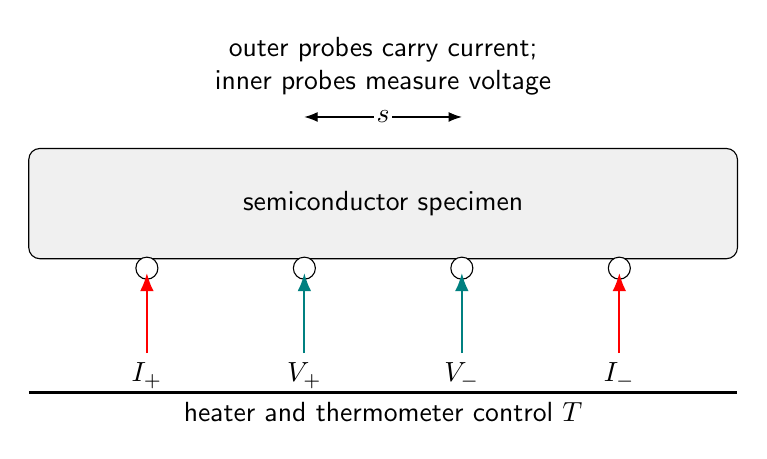
\begin{tikzpicture}[font=\sffamily,>=Latex]
\draw[fill=gray!12,rounded corners] (0,0) rectangle (9,1.4);
\node at (4.5,.7) {semiconductor specimen};
\foreach \x/\lab/\col in {1.5/$I_+$ /red,3.5/$V_+$ /teal,5.5/$V_-$ /teal,7.5/$I_-$ /red}{
  \draw[fill=white] (\x,-.12) circle (.14);
  \draw[thick,\col,-Latex] (\x,-1.2)--(\x,-.18);
  \node[below] at (\x,-1.2) {\lab};
}
\draw[<->] (3.5,1.8)--node[fill=white,inner sep=1pt] {$s$}(5.5,1.8);
\node[align=center] at (4.5,2.45) {outer probes carry current;\\inner probes measure voltage};
\draw[thick] (0,-1.7)--(9,-1.7);
\node[below] at (4.5,-1.7) {heater and thermometer control $T$};
\end{tikzpicture}
\end{document}
